\documentclass[final]{article}

\usepackage{amsmath}
\usepackage{amsfonts}
\usepackage{graphicx}
\usepackage{caption}
\usepackage{subcaption}
\usepackage{booktabs}
\usepackage{url}
\usepackage{color}

\title{Classifying brain states induced by complex visual stimuli}

\author{Andrew Floren\\
1 University Station, C0803\\
The University of Texas at Austin\\
Austin TX, 78712-1084 USA\\
afloren@mail.utexas.edu\\
(214) 384-2895\\}

\date{}

\bibliographystyle{acm}

\begin{document}

\maketitle

\begin{abstract}
abstract
\end{abstract}

\section{Introduction}
In traditional fMRI experiments, investigators seek to identify relationships between the measured BOLD signal and a carefully designed stimulus in order to tease out the purpose of particular brain regions.
Recently, a new trend has developed where researchers are instead looking to predict what stimulus was presented given the measured BOLD signal \cite{Haxby2001,Mitchell2003,Haynes2006}.
While successful, most of these experiments involve presenting static images from a limited number classes such as faces and places.
Then, the researchers try to classify which image or class of images was presented during each frame by analyzing the measured BOLD signal using machine learning classifiers.
While this has proven to be a successful approach, it does not mimic the dynamic environment in which brains have evolved.
Our goal is to analyze brain function with dynamically changing stimuli that portray real world experiences.
Further, we were interested to see what information could be gleaned from the BOLD signal beyond object categories.
We used virtual world technology to specify the stimuli in detail.
Given our long-term interest in PTSD, we created a virtual town intended to suggest the kinds of real-world settings currently encountered by our military forces.
Virtual character representing friendly forces and hostile combatants were presented in a virtual town.
We then trained linear SVMs (support vector machines) and feed forward neural networks to predict the number of characters in each stimulation.
[Bruce: this is most of your introduction from the abstract but feel free to rewrite the whole thing. I'll add in the literature review once you are happy with the introduction.]

\section{Methods}

\subsection{Subjects}
Five male adults, with normal or corrected to normal vision, participated in the experiments. 
All subjects participated in three sessions, two sessions to collect machine-learning data, and one session to measure a high-resolution volume anatomy. 
Informed consent was obtained from all subjects.

\subsection{Stimulus}
We developed a virtual reality environment similar to many popular first person video games using the Unreal Engine 2 SDK \cite{UnrealEngine2}.
The stimuli is dynamically rendered and presented from the point of view of a camera moving through this 
virtual environment using a block design. First, the viewpoint moves for 15 seconds through the virtual 
environment with no characters present (Fig. \ref{fig:stimulus}(a)), then pauses for 15 seconds during 
which a group of characters fades into view (Fig. \ref{fig:stimulus}(b)). Each run consists of 12 
alternations between moving through the virtual environment and character presentations. 
In each scanning session, 4 to 6 runs were collected.

The camera is constantly moving (even during the character presentation periods the camera slowly pans and rotates) and the characters are animated so that the presented scene is never static.
The number and location of characters varies with each presentation in a quasi-random fashion.
The number of characters presented varied from 1 to 6.
A presentation with a particular number of characters appears twice in each run, however the order of these presentations was randomized.
It should be noted that this random ordering was generated once and held constant between subjects.
Additionally, even between character presentations with the same number of characters, the locations of those characters varies considerably; compare Fig. \ref{fig:stimulus} (b) and (c).
[I need another frame from the stimulus to illustrate this point. These figures are all from the original report but I'd like to generate new ones if I can get access to a machine with the stimulus.]

\begin{figure}[!htbp]
\centering
\begin{subfigure}[t]{0.3\textwidth}
\centering
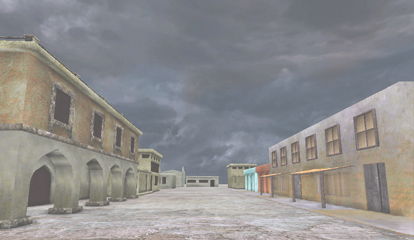
\includegraphics[width=\textwidth]{figures/stimulus-movement}
\caption{}
\label{fig:stimulus-movement}
\end{subfigure}
\begin{subfigure}[t]{0.3\textwidth}
\centering
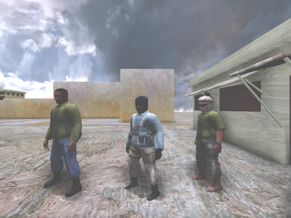
\includegraphics[width=\textwidth]{figures/stimulus-characters}
\caption{}
\label{fig:stimulus-characters}
\end{subfigure}
\begin{subfigure}[t]{0.3\textwidth}
\centering
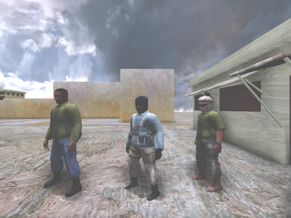
\includegraphics[width=\textwidth]{figures/stimulus-location}
\caption{}
\label{fig:stimulus-location}
\end{subfigure}
\caption{
\ref{fig:stimulus-movement} An example frame from the stimulus while the camera is moving through the virtual envronment. 
\ref{fig:stimulus-characters} An example frame from the stimulus while characters are being presented.
\ref{fig:stimulus-location} Another example frame from the stimulus while characters are being presented.
Note how the locations of the characters varies considerably between these two frames.
[I'm still playing around with finding the best way to present and reference subfigures.]}
\label{fig:stimulus}
\end{figure}

\subsection{MRI protocols}
Imaging was performed an GE Signa Excite HD scanner using the product 8-channel head coil.
We collected whole-brain image volumes using a custom GRAPPA-accelerated EPI sequence \cite{newbold}. 
Sequence parameters were g-factor = 2,  TE = 25 ms, TR = 2.5 s, and  2.5-mm cubic voxels across a 200 mm field-of-view. 
The slice prescription included 40 slices oriented along the AC-PC axis (Fig. \ref{fig:rx}). 
A high-order shim was  performed to improve field homogeneity.

A set of T1-weighted structural images was obtained on the same prescription at the end of each machine-learning session using a three-dimensional (3D) RF-spoiled GRASS (SPGR) sequence. 
These anatomical images were then used to align the functional data to a structural 3D reference volume, which was acquired for each subject in a separate session. 
The structural reference volume was T1-weighted with good gray-white contrast and was acquired using a 3D, inversion-prepared, SPGR sequence (minimum TE and TR, TI = 450 ms, 15° flip angle, isometric voxel size of 0.7 mm, 2 excitations, ~28-minimum duration).

\begin{figure}[!htbp]
\centering
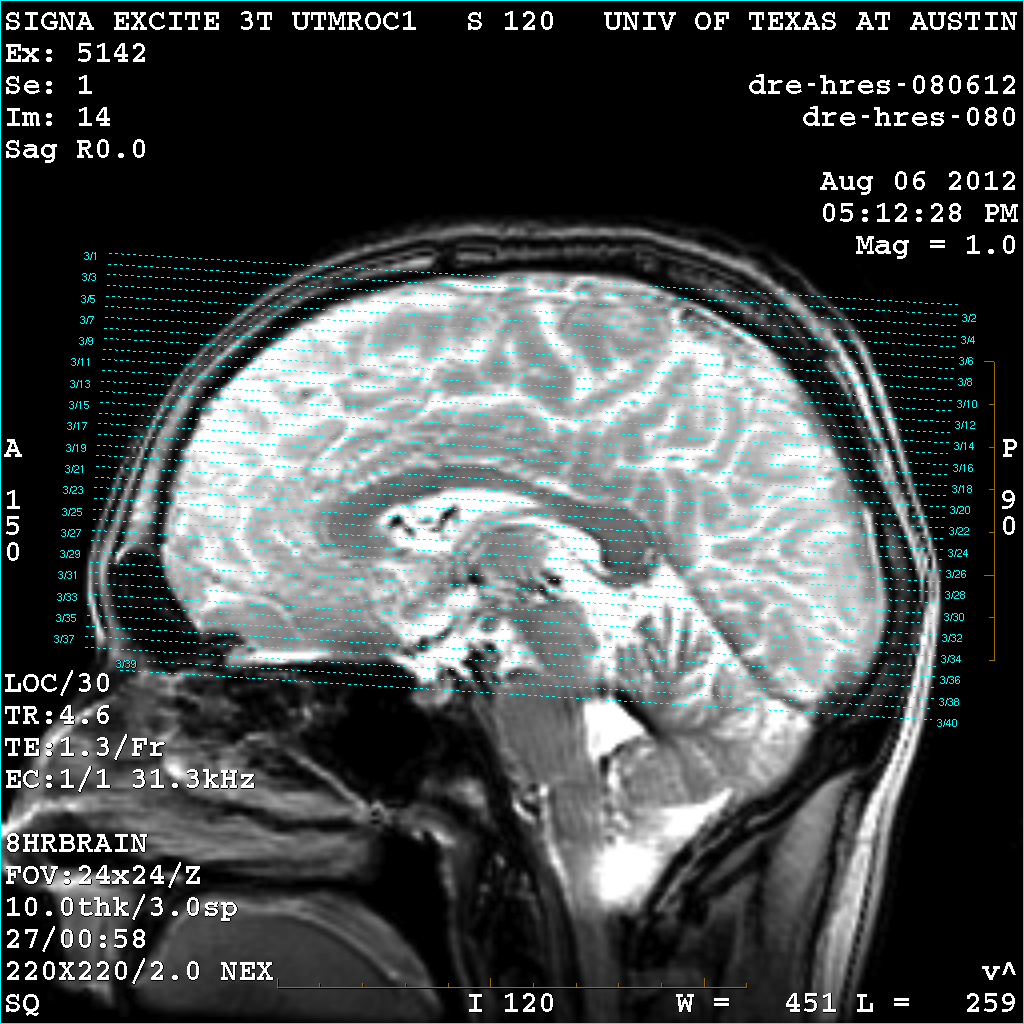
\includegraphics[width=0.5\textwidth]{figures/rx}
\caption{An example prescription from one of the subjects.}
\label{fig:rx}
\end{figure}

\subsection{Preprocessing}
Preprocessing of the fMRI data was performed using the mrVista software package (available for download at \url{http://vistalab.stanford.edu/}) as well as additional tools developed on the mrVista framework in our lab. 
The first 15 seconds seconds of data  were discarded fto reduce transient effects.
We then estimated in-scan motion using a robust scheme \cite{Nestares and Heeger 2000}. 
Between-run motion was corrected using the same intensity-based scheme, this time applied to the temporal average intensity of the entire scan. 
The last run of the session was used as the reference. 
Additionally, we applied a Wiener filter deconvolution \cite{Wiener} using a generic difference-of-gamma HRF \cite{Glover} to shift the peak response in time so that it is aligned with its associated stimulus.

Wiener filter deconvolution can be summarized as follows:
Given a system
\begin{equation}
y(t) = h(t) \ast x(t) + n(t)
\end{equation}
where $x(t)$ is the signal of interest, $h(t)$ is some blurring kernel, $n(t)$ is independent additive noise, and $y(t)$ is the recorded signal.
We want to find the deconvolution kernel $g(t)$ such that 
\begin{equation}
\hat{x}(t) = g(t) \ast y(t)
\end{equation}
minimizes the mean squared error between $x(t)$ and $\hat{x}(t)$, or
\begin{equation}
\sum_{t}{\left( \hat{x}(t) - x(t) \right)^{2}}
\end{equation}
The solution for the optimal $g(t)$ is most easily expressed in the Fourier domain.
\begin{equation}
g(t) \xrightarrow{\mathcal{F}} \frac{H^{*}(f)}{\left|H(f)^{2}\right| + \mbox{SNR}^{-1}(f)}
\end{equation}
Where $\mbox{SNR}(f)$ is the signal to noise ratio $\frac{\left| X(f) \right|}{\left| N(f) \right|}$ at frequency $f$.

In fMRI, $y(t)$ is the recorded BOLD signal, $h(t)$ is the hemodynamic response function, and $x(t)$ is the neuronal population response.
Calculating $g(t)$ requires estimates of the power spectral density of the signal of interest as well as the noise.
However, the noise $n(t)$ corresponds not only to scanner noise but other nuisance factors such as pulse and respiration.
This makes modeling the noise, and its power spectral density, very difficult.
Therefore, we set $\mbox{SNR}(f) = 1$ for all frequencies $f$.
The primary effect of the resulting deconvolution is to shift the time series according to the delay caused by the hemodynamic response.
Figure \ref{fig:wiener-deconvolution} illustrates the effects of this deconvolution on a simple square wave as well as an example voxel time series.

\begin{figure}[!htbp]
\centering

\includegraphics[width=0.5\textwidth]{figures/placeholder}
\caption{(1) The difference-of-gamma HRF employed as $h(t)$. (2) The deconvolution kernel $g(t)$ calculated from $h(t)$. (3) A simple square wave. (4) The same square wave after convolution with $g(t)$. (5) An example voxel time series. (6) The same time series after convolution with $g(t)$.}
\label{fig:data-split}
\end{figure}

The high-resolution reference anatomies were segmented using the FreeSurfer analysis package 
\cite{FreeSurfer} to create approximate masks of the gray matter in each subject, as well as 
a surface model useful for visualization of the results.

\subsection{Dimensionality reduction}
We reduce the dimensionality of the problem by masking out a subset of the volume using a harmonic power analysis based upon the block design of our stimulus. 
It is straightforward to show that the spectral response of any linear system to a blocked alternation at frequency f will contain power only at f and its harmonics. 
Under a linear response assumption, we can therefore form an unbiased estimate of the response power by summing the power at these frequencies. 
Let $y(t)$ be the recorded discrete time series at some voxel.
Then let $Y(f)$ be the discrete Fourier transform of $y(t)$.
The harmonic power of that time series is defined as:
\begin{equation}
\frac{\sum_{i = 1}^{M}{\left|Y(i \cdot N)\right|^{2}}}{\sum_{f}{\left|Y(f)\right|^{2}}}
\end{equation}
Where $M$ is the number of harmonics and $N$ is the frequency of interest, in our case the period of the block alternations. 
Because the BOLD response has a predominantly low-pass temporal frequency response, we chose $M = 4$. 
Using this metric, we then selected a particular number N (range 1000-3000) voxels with the greatest power. 
This harmonic-power selection was based on the alternation between characters present and characters 
absent, without regard to the number of characters presented. Therefore, we will only be presenting 
classifier accuracy estimates for character count, and not for the presence or absence of 
characters to avoid cross-contamination between dimension-reduction and  classification criteria that 
would result in inflated classifier performance estimates \cite{CrossContamination}.

\subsection{Classification}
Using the time series from the voxels selected by the harmonic power analysis, we trained a linear SVM and a feed forward neural network.
These algorithms were trained and validated using a cross-fold approach \cite{Kohavi1995}.
To maximize our temporal resolution, each frame (point in the pre-processed time series) was treated 
as a separate data value, rather than  of averaging across the block as has been  done in previous work 
[give references].

[Should I introduce the concept of training, validation and test sets here?] [Yes]

Previous studies have discussed issues with optimistic performance estimates due to temporal correlations violating independence assumptions between training and test set examples \cite{Pereira2009}.
We were interested in more closely examining the relationship between performance estimates and this temporal correlation.
To accomplish this, we estimated classifier performance using 5 different methods for splitting the 
training and test examples in order to vary the average temporal delay between frames in the training 
and test sets. The first four methods deal only with frames from a particular session.
In the first method, which we will refer to as the frame split, frames were independently drawn into the 
training and test sets. Although the draws were independent, there is no restriction to prevent adjacent 
frames being split between the training and test sets.
In the second method, which we will refer to as the block split, sets of frames corresponding to the 
various stimulus blocks were independently drawn into the training and test sets.
Our stimulus design enables us to break runs into two sets that each contain a complete set of 
character-number presentations. Accordingly, in our third method, which we will refer to as half-run 
split, sets of frames were independently drawn from these half-runs. Similarly, in our fourth method, 
termed run split, entire runs of frames were independently drawn. For the fifth method, termed session
split, we used a single entire session for training and a second session for test.
This method is similar to measures of between-session classifier accuracy used previously [give refs].
Table \cite{tempSplitTable} summarizes these temporal-split methods and the mean temporal delay between the 
training and test data, which varies from ~30 s (frame split) to several months (session split).

For the frame and block splits, the classifier performances were estimated using 10-fold cross-validation.
That is, the dataset was randomly split into the training and test sets 10 times and a classifier is trained on each split.
The classifier's performance is then estimated as the average of its performance across all 10 splits.
For the half-run, run, and session splits, only 8, 4, and 2 unique splits are possible, respectively, due to 
the much smaller number of runs and sessions per subject. Therefore, only 8-fold, 4-fold, and 2-fold 
cross-validation were employed for estimating classifier performance on these splits.

Classifier performance has been described by a number of metrics [refs]. In 
particular, one can define \it{precision} as [...details], and \it{recall} as 
[details...]. Here, the performance of each classifier was characterized by its micro-averaged
 $F$-measure \cite{Ozgur2005}. The $F$-measure for a single class is described by the following 
 equations:
\begin{equation}
\mbox{precision} = \frac{tp}{tp + fp}
\label{eqn:precision}
\end{equation}
\begin{equation}
\mbox{recall} = \frac{tp}{tp + fn}
\label{eqn:recall}
\end{equation}
\begin{equation}
F = 2 \cdot \frac{\mbox{precision} \cdot \mbox{recall}}{\mbox{precision} + \mbox{recall}}
\label{eqn:f1}
\end{equation}
Where $tp$ is the number of true positives, $fp$ is the number of false positives, and $fn$ is the number of false negatives.
The $F$-measure is a more robust measure of the performance of a classifier than either precision or recall alone.
For example, if the classifier labeled everything as positive then the recall would be perfect but the precision would be at chance levels.
On the other hand, if the classifier only labeled examples it was highly confidant in as positive then precision would be high but recall would be low.
The $F$-measure can be generalized for multiple classes by summing true positive, false positive, and false negative counts across all classes.
\begin{equation}
\mbox{precision}_{avg} =\frac{\sum_{i}^{M}{tp_{i}}}{\sum_{i}^{M}{\left( tp_{i} + fp_{i} \right)}}
\end{equation}
\begin{equation}
\mbox{recall}_{avg} = \frac{\sum_{i}^{M}{tp_{i}}}{\sum_{i}^{M}{\left( tp_{i} + fn_{i} \right)}}
\end{equation}
Where $M$ is the number of classes. [You used M for harmonic numbers before; use some other symbol]
The multi-class $F$-measure is then calculated as:
\begin{equation}
F_{avg} = 2 \cdot \frac{\mbox{precision}_{avg} \cdot \mbox{recall}_{avg}}{\mbox{precision}_{avg} + \mbox{recall}_{avg}}
\end{equation}
This is known in the literature as the  micro-averaged $F$-measure.
It should be noted that in a symmetric multi-class scheme such as ours, the micro-averaged precision, 
recall, and $F$-measure will all be identical. [I don't understand this statement; why are we not just using recall in that case?]

Another convenient tool for examining classifier performance is the confusion matrix.
If $\mathbf{C}$ is a confusion matrix, then the value of $C_{ij}$ is equal to the number examples of class $i$ that were classified as class $j$.
Therefore, values along the diagonal of a confusion matrix correspond to correct classifications while other values correspond to incorrect classifications.
The confusion matrix also simplifies calculating precision and recall for each class.
The value of $C_{ii}$ divided by the sum of all values along row $i$ is the recall of the $i^{th}$ class.
Similarly, the value of $C_{jj}$ divided by the sum of all values along column $j$ is the precision of the $j^{th}$ class.
Finally, the micro-averaged $F$-measure can be calculated by dividing the sum along the diagonal, or the trace, by the sum of the entire matrix.

\subsection{Sensitivity Analysis}
Non-linear multi-variate machine-learning classifiers can tell us whether the time-series data from a 
subset of human brain voxels is discriminative with respect to the task being predicted. However, these 
results do not show which voxels in the large group were actually important for that discrimination
This is important for localizing functions in the brain.
One existing technique is to train machine learning classifiers on small localized areas in the brain and use their performance as a measure of the strength of the function in question in that area.
While this technique is effective for simple highly localized functions, the results are less clear when the function is sparsely distributed over the brain.
No one region may contain enough information for accurate predictions.

To overcome this limitation, we have trained our classifiers on large regions of the brain and used sensitivity analysis to attempt to tease out the sparsely distributed voxels that are relevant for task discrimination.
Specifically, we calculate the sensitivity, or magnitude of change, of the output of the classifier with respect to a change in each voxel.
In feed forward neural networks, this problem has been well explored \cite{Zurada1994}.
Let $\mathbf{o}$ be the vector of outputs and $\mathbf{x}$ be the vector of inputs.
Then the sensitivity of output $k$ to input $i$ is defined by:
\begin{equation}
S_{ki} = \frac{\delta o_{k}}{\delta x_{i}}
\end{equation}
Or simply, the partial derivative of the output with respect to the input.
If we let $\mathbf{w}$ be the weight matrix from the hidden layer to the output layer and $\mathbf{v}$ be the weight matrix from the input layer to the hidden layer then the partial derivative can be expressed as follows:
\begin{equation}
\frac{\delta o_{k}}{\delta x_{i}} = o'_{k} \sum^{J}_{j=1}{w_{kj}y'_{j}v_{ji}}
\end{equation}
Where $J$ is the total number of hidden neurons,  $o'_{k}$ is the value of the derivative of the activation function at output $k$, and $y'_{j}$ is the value of the derivative of the activation function at hidden neuron {j}.
Finally, the entire sensitivity matrix can be expressed in matrix notation as:
\begin{equation}
\mathbf{S} = \mathbf{O}' \times \mathbf{W} \times \mathbf{Y}' \times \mathbf{V}
\end{equation}
Where
\begin{equation}
\mathbf{O}' = diag(o'_{1},~o'_{2},~\cdots,~o'_{K})
\end{equation}
\begin{equation}
\mathbf{Y}' = diag(y'_{1},~y'_{2},~\cdots,~y'_{K})
\end{equation}
However, because the transfer functions are non-linear they can only be evaluated for specific input values.
Therefore, we calculate the average sensitivity matrix across all input vectors.
\begin{equation}
\mathbf{S}_{avg} = \sqrt{ \frac{ \sum_{n = 1}^{N}{ \left( \mathbf{S}^{n}\right)^{2} } }{N} }
\end{equation}
Where $N$ is the number of input vectors.
The magnitude is squared to avoid problems with positive and negative sensitivities canceling out when averaging.
The average of the absolute value of sensitivities could also be employed.
This still gives a sensitivity value for each voxel with respect to every output, whereas it is useful to have a measure of the sensitivity of a voxel with respect to any output.
To calculate this number we simply take the maximum sensitivity of each voxel across all outputs.
\begin{equation}
\Phi_{i} = \max_{k=1 \dots K}{S_{ki,~avg}}
\end{equation}
This sensitivity can now be projected back into the volume anatomy space to create an activation map.
Further, this sensitivity can also be used to reduce the dimensionality of the machine learning classifier by retraining the algorithms using only the voxels that had a sensitivity over some threshold.

\section{Results}
Table \ref{tab:results} contains the cross-validated $F$-measures of the linear SVM and feed forward neural networks for all 5 subjects and all 5 training and test split methods.
There is some variation of classifier performance between subjects, but in all cases the performance is well above chance. 
These variations between subjects could be the result of differences in age, general cognitive state, or simply how much attention the subject was paying to the stimulus during the scan.
It is evident that as the average temporal distance between data in the training and test sets increases, the estimated performance of the classifiers decreases.
This relationship is plotted in figure \ref{fig:performance-verse-temporal-distance}.
[I plan to calculate confidence values for this plot].

The average confusion matrix presented in figure \ref{fig:average-confusion} gives a more intuitive look at the performance of the classifier.
From this matrix we can see that the classifiers are much better at detecting the presence of a single character than any other count.
In fact, there are almost no cases of confusion between 1 and 2 characters.
Apparently, these two situations evoke very different responses in the brain.
The rest of the character counts are distinguished with relatively equal accuracy.
However, there is a slight tendency to mis-classify the 6 character presentation.
This could be a result of 6 characters being too much for the subject to consider individually.
Interestingly, the confusion is not often between 5 and 6 characters, but rather between 1 or 2 and 6 characters.
This would seem to indicate that when the number of characters grows too large, they are interpreted as a single unit.
It should also be noted that the majority of the incorrect responses lay just off the main diagonal.
These responses correspond to the classifier being wrong by a single character in its classification.
For example, the machine learning algorithm classified a frame as containing 4 characters when it only contained 3 characters.
The $F$-measure does not take the cardinality of the classes into account and considers mislabeling 1 character as 2 equivalent to mislabeling 1 character as 6 characters.
Figure \ref{figsoft-measure} presents a soft measure of accuracy for the two classifiers that takes the cardinality of the classes into consideration.

The sensitivity analysis of the feed forward neural network projected back into the anatomy volume is presented in figure \ref{sensitivity-analysis}.
[David: We need to make come comments on this figure related to neuroscience/brain mapping. We should look at the data to make sure this is true, but since we are still employing the same harmonic analysis the activated regions should be very similar to the original report.]
After aligning all of the subjects to the MNI template \ref{MNI} and combining these activation maps we found that the majority of activation took place in [need to do this analysis still].
This combined activation map is presented in figure \ref{fig:MNI-average-sensitivity}.

To better explore the relationship between sensitivity and classifier performance we plotted the performance of the classifier when trained on only a subset of the input voxels as determined by a minimum sensitivity cut off.
Figure \ref{fig:sensitivity-cutoff} shows this plot on top of the histogram of sensitivity values.
Interestingly, the performance of the classifier is not significantly affected until a majority of the voxels have been removed.
This would indicate that either only a small number of voxels are relevant for classification or that the information is highly redundant between voxels.
In actuality, it is likely a combination of the two.
The harmonic analysis will select some voxels that only appeared to covary with the stimulus presentation by chance.
These voxels will be assigned very low sensitivity values by the trained classifiers.
However, other voxels may actually covary with the stimulus but their patterns of activation may not be highly discriminative with respect to character count.
These voxels will also be assigned low sensitivity values by the trained classifiers.
Therefore, high sensitivity is sufficient but not necessary for the localization of a function in a particular region.

\begin{table}[!htbp]
\centering
\begin{tabular}{l *{10}{c}}
\toprule
& \multicolumn{2}{c}{Frame} & \multicolumn{2}{c}{Block} & \multicolumn{2}{c}{Half-Run} & \multicolumn{2}{c}{Run} & \multicolumn{2}{c}{Session} \\
\cmidrule(lr){2-3} \cmidrule(rl){4-5} \cmidrule(rl){6-7} \cmidrule(rl){8-9} \cmidrule(l){10-11}
Subject	& SVM & NN & SVM & NN & SVM & NN & SVM & NN & SVM & NN \\
\midrule
A		& 0.6 & 0.6 & 0.6 & 0.6 & 0.6 & 0.6 & 0.6 & 0.6 & 0.6 & 0.6 \\
B		& 0.6 & 0.6 & 0.6 & 0.6 & 0.6 & 0.6 & 0.6 & 0.6 & 0.6 & 0.6 \\
C		& 0.6 & 0.6 & 0.6 & 0.6 & 0.6 & 0.6 & 0.6 & 0.6 & 0.6 & 0.6 \\
D		& 0.6 & 0.6 & 0.6 & 0.6 & 0.6 & 0.6 & 0.6 & 0.6 & 0.6 & 0.6 \\
E		& 0.6 & 0.6 & 0.6 & 0.6 & 0.6 & 0.6 & 0.6 & 0.6 & 0.6 & 0.6 \\
Average	& 0.6 & 0.6 & 0.6 & 0.6 & 0.6 & 0.6 & 0.6 & 0.6 & 0.6 & 0.6 \\
\bottomrule 
\end{tabular}

\caption{The multi-class $F$-measures of the linear SVM and the feed forward neural network after cross-validation for all 5 subjects and all 5 training and test split methods. }
\label{tab:results}
\end{table}

\begin{figure}[!htbp]
\centering

\includegraphics[width=0.5\textwidth]{figures/placeholder}
\caption{The average performance of the SVM and neural network classifiers plotted against the average temporal distance between data in the training and test sets.}
\label{fig:performance-verse-temporal-distance}
\end{figure}

\begin{figure}[!htbp]
\centering
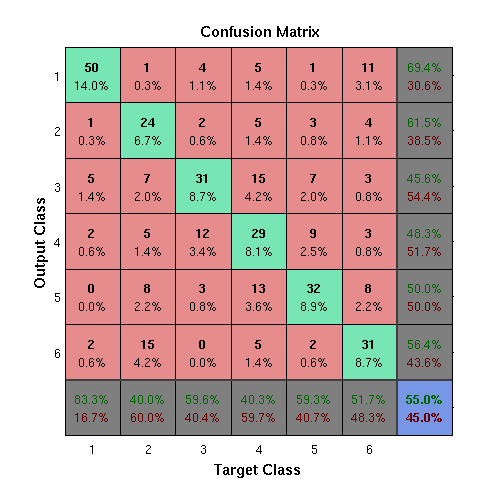
\includegraphics[width=0.5\textwidth]{figures/confusion-average}
\caption{The average confusion matrix across all subjects when the train, test, and validation sets were divided by block.}
\label{fig:average-confusion}
\end{figure}

\begin{figure}[!htbp]
\centering

\includegraphics[width=0.5\textwidth]{figures/placeholder}
\caption{The average performance of the linear SVM and feed forward neural network using a soft measure of accuracy.}
\label{fig:soft-measure}
\end{figure}

\begin{figure}[!htbp]
\centering
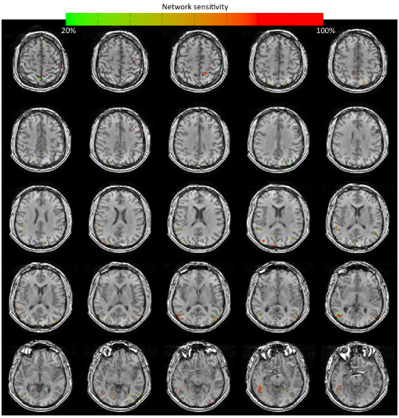
\includegraphics[width=0.5\textwidth]{figures/sensitivity-analysis}
\caption{The results of the sensitivity analysis mapped back on to the volume anatomy.}
\label{fig:sensitivity-analysis}
\end{figure}

\begin{figure}[!htbp]
\centering

\includegraphics[width=0.5\textwidth]{figures/placeholder}
\caption{The average sensitivity analysis of all subjects mapped onto the slightly inflated MNI template brain.}
\label{fig:MNI-average-sensitivity}
\end{figure}

\begin{figure}[!htbp]
\centering
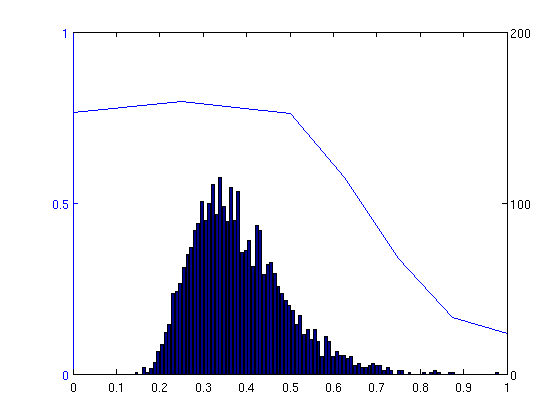
\includegraphics[width=0.5\textwidth]{figures/sensitivity-cutoff}
\caption{A histogram of the sensitivity analysis values and a plot of the feed forward neural network $F_1$ score when the inputs are pruned at a particular sensitivity value. }
\label{fig:sensitivity-cutoff}
\end{figure}

\section{Discussion}
[The conclusion is still mostly pulled from the HBM abstract. I would like to rewrite this after the rest of the paper is more complete. Especially with regards to future research directions.]

The reported results are well above chance, indicating there is useful information about character number in the BOLD signal.
The sensitivity analysis indicates that no single region of the brain is responsible for counting characters, and there is not a simple linear relationship between magnitude of activation and cardinality.
Rather, it is a complex pattern of distributed activation requiring machine learning methods to capture the stimulus-response relationship.

Earlier, we presented this new trend in brain sate classification as a departure from traditional fMRI experiments which seek to identify the purpose or function of particular brain regions.
However, it is important to note that through sensitivity analysis these machine learning classifiers can be re-purposed for just that goal.
If a region of the brain is highly important for accurately predicting the presence of a particular stimulus then it logically follows that that region must somehow be involved in the processing of that stimulus.
Furthermore, multi-voxel non-linear machine learning classifiers can potentially identify much more complex interactions between brain regions than the simple GLM.


\bibliography{bib}

\end{document}
